%%%%%%%%%%%%%%%%%%%%%%%%%%%%%%%%%%%%%%%%%
% Lachaise Assignment
% LaTeX Template
% Version 1.0 (26/6/2018)
%
% This template originates from:
% http://www.LaTeXTemplates.com
%
% Authors:
% Marion Lachaise & François Févotte
% Vel (vel@LaTeXTemplates.com)
% Minor improvements by Galimba - 2020
%
% License:
% CC BY-NC-SA 3.0 (http://creativecommons.org/licenses/by-nc-sa/3.0/)
% 
%%%%%%%%%%%%%%%%%%%%%%%%%%%%%%%%%%%%%%%%%

%----------------------------------------------------------------------------------------
%	PACKAGES AND OTHER DOCUMENT CONFIGURATIONS
%----------------------------------------------------------------------------------------

\documentclass{article}

%%%%%%%%%%%%%%%%%%%%%%%%%%%%%%%%%%%%%%%%%
% Lachaise Assignment
% Structure Specification File
% Version 1.0 (26/6/2018)
%
% This template originates from:
% http://www.LaTeXTemplates.com
%
% Authors:
% Marion Lachaise & François Févotte
% Vel (vel@LaTeXTemplates.com)
% Minor improvements by Galimba - 2020
%
% License:
% CC BY-NC-SA 3.0 (http://creativecommons.org/licenses/by-nc-sa/3.0/)
% 
%%%%%%%%%%%%%%%%%%%%%%%%%%%%%%%%%%%%%%%%%

%----------------------------------------------------------------------------------------
%	PACKAGES AND OTHER DOCUMENT CONFIGURATIONS
%----------------------------------------------------------------------------------------

\usepackage{amsmath,amsfonts,stmaryrd,amssymb} % Math packages

\usepackage{enumerate} % Custom item numbers for enumerations

\usepackage[ruled]{algorithm2e} % Algorithms

\usepackage[framemethod=tikz]{mdframed} % Allows defining custom boxed/framed environments
\usepackage{hyperref}
\usepackage{xcolor}
\definecolor{medium-blue}{rgb}{0,0,1}
\hypersetup{colorlinks, urlcolor={medium-blue}}
\usepackage{listings} % File listings, with syntax highlighting
\lstset{
	basicstyle=\ttfamily, % Typeset listings in monospace font
}
\usepackage{fancyhdr}
%----------------------------------------------------------------------------------------
%	DOCUMENT MARGINS
%----------------------------------------------------------------------------------------
\pagestyle{fancy}
\fancyhf{}
%\rhead{PRELIMINARY REPORT V1.0}
\usepackage{geometry} % Required for adjusting page dimensions and margins

\geometry{
	paper=a4paper, % Paper size, change to letterpaper for US letter size
	top=2.5cm, % Top margin
	bottom=3cm, % Bottom margin
	left=2.5cm, % Left margin
	right=2.5cm, % Right margin
	headheight=14pt, % Header height
	footskip=1.5cm, % Space from the bottom margin to the baseline of the footer
	headsep=1.2cm, % Space from the top margin to the baseline of the header
	%showframe, % Uncomment to show how the type block is set on the page
}

%----------------------------------------------------------------------------------------
%	FONTS
%----------------------------------------------------------------------------------------

\usepackage[utf8]{inputenc} % Required for inputting international characters
\usepackage[T1]{fontenc} % Output font encoding for international characters

\usepackage{XCharter} % Use the XCharter fonts

\usepackage{xcolor}
%----------------------------------------------------------------------------------------
%	COMMAND LINE ENVIRONMENT
%----------------------------------------------------------------------------------------

% Usage:
% \begin{commandline}
%	\begin{verbatim}
%		$ ls
%		
%		Applications	Desktop	...
%	\end{verbatim}
% \end{commandline}

\mdfdefinestyle{commandline}{
	leftmargin=10pt,
	rightmargin=10pt,
	innerleftmargin=15pt,
	middlelinecolor=black!50!white,
	middlelinewidth=2pt,
	frametitlerule=false,
	backgroundcolor=black!5!white,
	frametitle={Command Line},
	frametitlefont={\normalfont\sffamily\color{white}\hspace{-1em}},
	frametitlebackgroundcolor=black!50!white,
	nobreak,
}

% Define a custom environment for command-line snapshots
\newenvironment{commandline}{
	\medskip
	\begin{mdframed}[style=commandline]
}{
	\end{mdframed}
	\medskip
}

%----------------------------------------------------------------------------------------
%	FILE CONTENTS ENVIRONMENT
%----------------------------------------------------------------------------------------

% Usage:
% \begin{file}[optional filename, defaults to "File"]
%	File contents, for example, with a listings environment
% \end{file}

\mdfdefinestyle{file}{
	innertopmargin=1.6\baselineskip,
	innerbottommargin=0.8\baselineskip,
	topline=false, bottomline=false,
	leftline=false, rightline=false,
	leftmargin=2cm,
	rightmargin=2cm,
	singleextra={%
		\draw[fill=black!10!white](P)++(0,-1.2em)rectangle(P-|O);
		\node[anchor=north west]
		at(P-|O){\ttfamily\mdfilename};
		%
		\def\l{3em}
		\draw(O-|P)++(-\l,0)--++(\l,\l)--(P)--(P-|O)--(O)--cycle;
		\draw(O-|P)++(-\l,0)--++(0,\l)--++(\l,0);
	},
	nobreak,
}

% Define a custom environment for file contents
\newenvironment{file}[1][File]{ % Set the default filename to "File"
	\medskip
	\newcommand{\mdfilename}{#1}
	\begin{mdframed}[style=file]
}{
	\end{mdframed}
	\medskip
}

%----------------------------------------------------------------------------------------
%	NUMBERED QUESTIONS ENVIRONMENT
%----------------------------------------------------------------------------------------

% Usage:
% \begin{question}[optional title]
%	Question contents
% \end{question}

\mdfdefinestyle{question}{
	innertopmargin=1.2\baselineskip,
	innerbottommargin=0.8\baselineskip,
	roundcorner=5pt,
	nobreak,
	singleextra={%
		\draw(P-|O)node[xshift=1em,anchor=west,fill=white,draw,rounded corners=5pt]{%
		Question \theQuestion\questionTitle};
	},
}

\newcounter{Question} % Stores the current question number that gets iterated with each new question

% Define a custom environment for numbered questions
\newenvironment{question}[1][\unskip]{
	\bigskip
	\stepcounter{Question}
	\newcommand{\questionTitle}{~#1}
	\begin{mdframed}[style=question]
}{
	\end{mdframed}
	\medskip
}

%----------------------------------------------------------------------------------------
%	WARNING TEXT ENVIRONMENT
%----------------------------------------------------------------------------------------

% Usage:
% \begin{warn}[optional title, defaults to "Warning:"]
%	Contents
% \end{warn}

\mdfdefinestyle{warning}{
	topline=false, bottomline=false,
	leftline=false, rightline=false,
	nobreak,
	singleextra={%
		\draw(P-|O)++(-0.5em,0)node(tmp1){};
		\draw(P-|O)++(0.5em,0)node(tmp2){};
		\fill[black,rotate around={45:(P-|O)}](tmp1)rectangle(tmp2);
		\node at(P-|O){\color{white}\scriptsize\bf !};
		\draw[very thick](P-|O)++(0,-1em)--(O);%--(O-|P);
	}
}

% Define a custom environment for warning text
\newenvironment{warn}[1][Warning:]{ % Set the default warning to "Warning:"
	\medskip
	\begin{mdframed}[style=warning]
		\noindent{\textbf{#1}}
}{
	\end{mdframed}
}

%----------------------------------------------------------------------------------------
%	INFORMATION ENVIRONMENT
%----------------------------------------------------------------------------------------

% Usage:
% \begin{info}[optional title, defaults to "Info:"]
% 	contents
% 	\end{info}

\mdfdefinestyle{info}{%
	topline=false, bottomline=false,
	leftline=false, rightline=false,
	nobreak,
	singleextra={%
		\fill[black](P-|O)circle[radius=0.4em];
		\node at(P-|O){\color{white}\scriptsize\bf i};
		\draw[very thick](P-|O)++(0,-0.8em)--(O);%--(O-|P);
	}
}

% Define a custom environment for information
\newenvironment{info}[1][Info:]{ % Set the default title to "Info:"
	\medskip
	\begin{mdframed}[style=info]
		\noindent{\textbf{#1}}
}{
	\end{mdframed}
}

\usepackage{graphicx}
\graphicspath{ {./img/} } % Include the file specifying the document structure and custom commands

%----------------------------------------------------------------------------------------
%	ASSIGNMENT INFORMATION
%----------------------------------------------------------------------------------------

\title{rLending White Paper v1.0} % Title

\author{The rLending Dev Team\\ \texttt{support@rlending.app}} % Author name and email address

\date{ \today} % University, school and/or department name(s) and a date

%----------------------------------------------------------------------------------------

\begin{document}

\maketitle % Print the title

%----------------------------------------------------------------------------------------
%	ABSTRACT
%----------------------------------------------------------------------------------------

\section*{Abstract} 

We introduce an algorithmic distributed protocol that establishes autonomously regulated liquidity pools with interest rates derived from supply and demand. In this model, lenders earn revenue in exchange for their supplied assets and borrowers pay interests for the assets they used.

DEFI (Decentralized Finance) platforms are taking over the blockchain scene. They are predicated on the tenants of non-custodial, trust-less and secure systems with 100\% up-time.
\\ \\
This means:
\begin{itemize}
\item No single entity stores funds on behalf of the users.
\item Users are not required to wait long times for someone to process their transactions.
\item Transactions are highly secure (thanks to open protocols and independent auditors).
\item 24/7 accessibility from anywhere in the world.
\end{itemize}
In other words, there is no central bank or government authority imposing rules on how to operate. Instead, the platform was designed to be completely self-regulating. This is achieved by programming the protocol using distributed \textit{Smart Contracts} deployed on the \textbf{RSK Network}\footnote{\href{https://www.rsk.co/}{The RSK Network}}. Smart contracts handle the majority of logic that has historically been handled by human inputs, vastly optimizing transaction time and cost.
\begin{center}
\noindent\rule{8cm}{0.4pt}
\end{center}

%----------------------------------------------------------------------------------------
%	INTRODUCTION
%----------------------------------------------------------------------------------------
\section*{Introduction}
Financial markets have had a difficult time keeping up with modern technologies and have stuck to a classic centralized model. In the last couple of years we have seen an increased awareness of the issues this presents. Demand has arisen for technologies that provide modern solutions \footnote{\href{https://blog.rsk.co/noticia/the-cutting-edge-of-sidechains-liquid-and-rsk/}{2016 article on pegged side-chains}} to issues such as facilitating investments and trade across blockchain platforms.

Classic Centralized Financial (\textit{CEFI}) systems are trust-based systems (users have to trust that the exchange won't get hacked, abscond with the user's assets, incorrectly close out a position or even suffer downtime). Users rely on centralized authorities to manage their assets and often have to trust that the protocols implemented are the same as the ones advertised.

To properly develop a Decentralized \textit{DEFI} ecosystem, \textbf{Open Finance}\footnote{\href{https://blog.rsk.co/noticia/open-finance-defi-rsk-a-definitive-guide/}{2020 article on Open Finance}} platforms must be deployed on the main blockchains, since those are the ones that move the most volume, thus increasing decentralization.

In this paper, we propose an algorithmic distributed protocol aiming to be deployed on the RSK network. Our main motivation is to allow users to lend crypto currencies as collateral and to borrow crypto-assets based on interest rates set by real-time supply and demand smart contracts.

\begin{center}
\noindent\rule{8cm}{0.4pt}
\end{center}

%----------------------------------------------------------------------------------------
%	ARCHITECTURE
%----------------------------------------------------------------------------------------
\section{Architecture}

The proposed solution would require several implementation layers. The next graph shows the abstract scheme.

\begin{center}
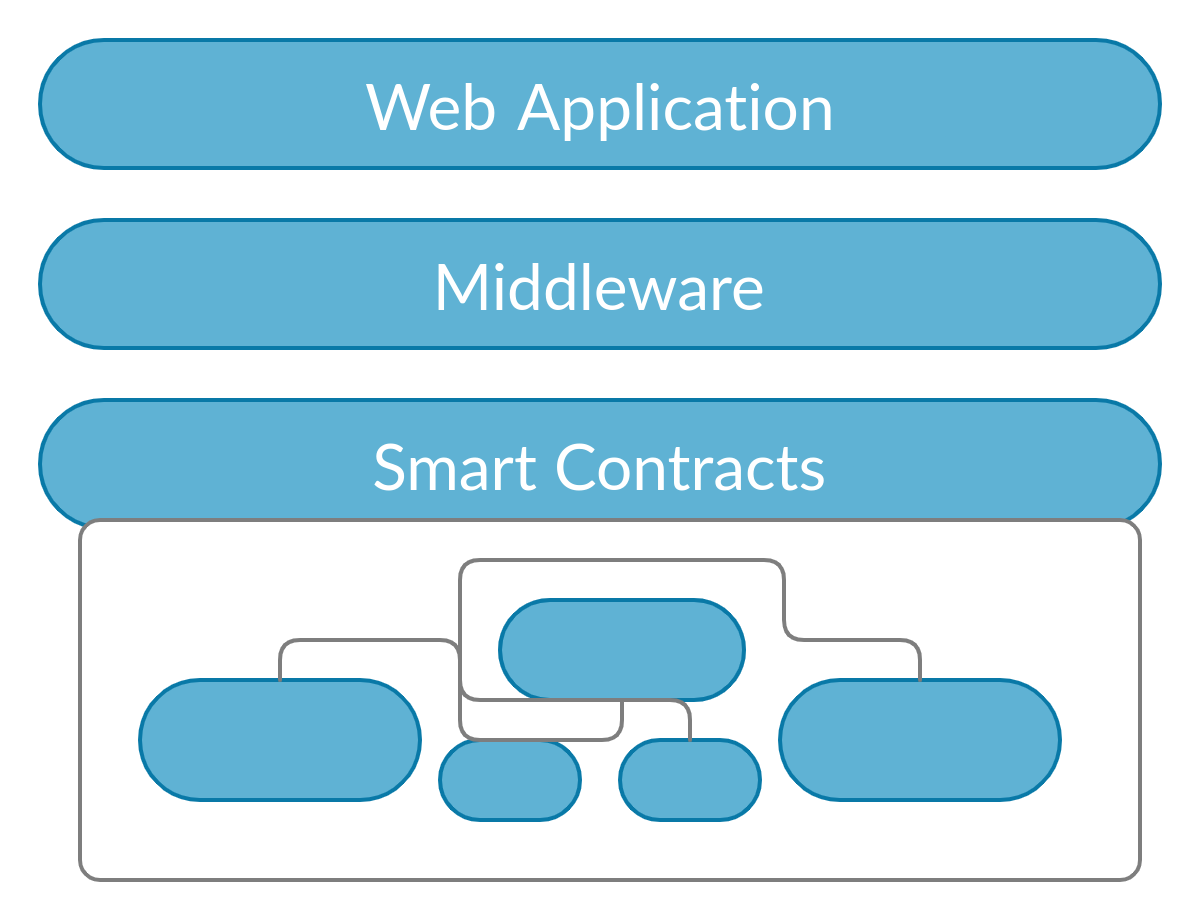
\includegraphics[width=8cm]{architecture.png}
\end{center}

We consider the top level to be the application layer, consisting of the \textbf{rLending User Interface}\footnote{\href{https://github.com/riflending/rlending-ui}{rLending User Interface source code}}.
\\
In contrast, the low-level layer composing the \textbf{rLending Protocol}\footnote{\href{https://github.com/riflending/rlending-protocol}{rLending protocol source code}}, is distributed (\textit{deployed}) as a set of smart contracts on the RSK Network.
\\ 
The middle layer is a custom made library that manages the interactions between the lower level (\textit{back-end}) and the top level (\textit{front-end}). This \textbf{middleware}\footnote{\href{https://github.com/riflending/rlending-ui/src/components/middleware}{rLending middleware source code}}, as the rest of the source code, is also publicly available and could be used to develop alternative applications to connect with the protocol, such as bots, alternative transaction explorers or automated liquidators.

%------------------------------------------------
\subsection{The rLending Protocol}

The \textbf{rLending protocol} establishes money markets, which are pools of assets with algorithmically derived interest rates, based on the supply and demand for the
crypto-asset. Suppliers (and borrowers) interact directly with the protocol, earning (and paying) a floating interest rate, without having to negotiate terms such as maturity, interest rate, or collateral with a peer or counterparty. 
Each money market is unique to an asset already in the \textbf{RSK Network} (such as rBTC, an ERC-20 stablecoin such as rKovDAI, or any ERC-20 compatible token such as RIF), and contains a transparent and publicly-inspectable ledger, with a record of all transactions and historical interest rates.

%------------------------------------------------
\subsubsection{Supplying}
Unlike an exchange or peer-to-peer platform, where a user's assets are matched and lent to another
user, the rLending protocol aggregates the supply of each user; when a user supplies an asset, it
becomes a fungible resource, effectively forming a liquidity pool. This approach offers significantly more liquidity than direct lending; unless every asset in a market is borrowed \textbf{(see below: the protocol incentivizes liquidity)}, users can withdraw their assets at any time, without waiting for a specific loan to mature.
\\
Assets supplied to a market are represented by an internal ERC-20 token balance (\textbf{“cToken”}), which entitles the owner to an increasing quantity of the underlying asset. As the money market accrues interest, which is a function of borrowing demand, cTokens become convertible into an increasing amount of the underlying asset. In this way, earning interest is as simple as holding \textbf{cTokens}\footnote{\href{https://test.rlending.app/doc/keyConcepts\#ctokens}{rLending cToken Documentation}}.

%------------------------------------------------
\subsubsection{Borrowing}

Using cTokens as collateral, the \textbf{rLending Protocol} allows users to frictionlessly borrow assets from the liquidity pools (\textit{markets}), for use anywhere in the RSK ecosystem. Unlike peer-to-peer protocols, borrowing from \textbf{rLending} simply requires a user to specify a desired asset; borrowing is instant and predictable. Similar to supplying an asset, each money market has a floating interest rate, set by market forces \textbf{(supply and demand)}, which determines the borrowing cost for each asset.

%------------------------------------------------
\subsubsection{Collateralization}
Assets held by users of the protocol, \textbf{represented by ownership of a cToken}, are used as collateral to borrow from the protocol. Each market has a \textbf{Collateral Factor}\footnote{\href{https://test.rlending.app/docs/keyConcepts\#ctokens}{rLending Collateral Factor Documentation}}, ranging from 0 to 1, that represents the portion of the supplied underlying asset value that can be borrowed. Illiquid, small-cap assets tend to have low collateral factors; they do not make good collateral, while liquid, high-cap assets have high collateral factors. The sum of the value of an account's underlying token balances, multiplied by the collateral factors, equals a user's \textbf{borrowing capacity}.
\\
\\
Users are able to borrow up to, but not exceeding, their borrowing capacity, and an account can
take no action (e.g. borrow, transfer cToken collateral, or redeem cToken collateral) that would
raise the total value of borrowed assets above their borrowing capacity; this protects the protocol
from default risk. Users should never borrow amounts close to their borrowing capacity, or else they run the risk of becoming prone to liquidation.

%------------------------------------------------
\subsubsection{Risk and liquidation}
If the value of an account's borrowing balance exceeds their borrowing capacity, a portion of
the outstanding borrowing may be repaid in exchange for the user's cToken collateral, at the current market price minus a liquidation discount (\textbf{Liquidation Factor}\footnote{\href{https://test.rlending.app/docs/keyConcepts\#liquidation}{rLending Liquidation Documentation}}; this incentives an ecosystem of arbitrageurs to quickly step in to reduce the borrower's exposure, and eliminate the protocol's risk.
\\ \\
Any rBTC address that possesses the borrowed asset may invoke the liquidation function, exchanging their asset for the borrower's cToken collateral. As both users, both assets and prices
are all contained within the \textbf{rLending protocol}, liquidation is frictionless and does not rely on any outside systems or managed order-books.

%------------------------------------------------
\subsection{The Interest Rate Model}
Rather than individual suppliers or borrowers having to negotiate over terms and rates, the \textbf{rLending protocol} utilizes an interest rate model that achieves an interest rate equilibrium, in each listed market, based on supply and demand. Following economic theory, interest rates (the “price” of money) should increase as a function of demand; when demand is low, interest rates should be low, and vice versa when demand is high. The utilization ratio \textbf{$U$} for each market \textbf{$\alpha$} unifies supply and demand into a single variable:
\begin{center}
$U_{a} = Borrows_{a} / (Cash_{a} + Borrows_{a})$
\end{center}
The demand curve is expressed as a function of utilization. As an example, borrowing interest rates may resemble the following:
\begin{center}
$Borrowing Interest Rate_{a}= 2.5\% + U_{a} * 20\%$
\end{center}
The interest rate earned by suppliers is implicit and is equal to the borrowing interest rate,
multiplied by the utilization rate.
\\ \\
\textbf{The protocol does not guarantee liquidity}; instead, it relies on the interest rate model to incentivize it. In periods of extreme demand for an asset, the liquidity of the protocol (the tokens available to withdraw or borrow) will decline; when this occur, interest rates rise, incentivizing supply and disincentivizing borrowing.

%------------------------------------------------
\subsection{Middleware layer}
We propose a custom middleware implementation based on \textbf{Ethers.js}\footnote{\href{https://ethers.io}{Ethers.js documentation}}. This layer is used to facilitate the interaction with the protocol, by providing an interface to the core functions. Some of the most interesting functions are listed here: \\

\begin{itemize}
\item \textbf{getMarkets(address)} returns the markets a user has entered as collateral.
\item \textbf{getCTokenMetadata(address)} fetches the metadata for a given cToken
\item \textbf{getAccountLiquidity(address)} queries the protocol and fetches the accounts liquidity or shortfall
\item \textbf{getTotalSupplysAndBorrows(address)} calculates the sum of all supplies and borrows for a given account
\item \textbf{getAccountHealth(address)} calculates the account health factor
\item \textbf{getAccountBalanceOfCtoken(address)} queries the cToken contract to fetch the account balance
\item \textbf{balanceOfUnderlying(address)} calculates the equivalent balance of underlying asset an account has
\item \textbf{getSupplyRate()} gets the current supply rate per block for a given market
\item \textbf{getBorrowRate()} gets the current borrow rate per block for a given market
\item \textbf{enterMarket() / exitMarket()} perform said functions for a given account in a given market, respectively
\item \textbf{getMaxWithdrawAllowed(address)} calculates the maximum amount of withdrawable assets an account may extract from the protocol
\item \textbf{supply(), borrow(), repay(), withdraw(), liquidate()}, etc..
\end{itemize}

We strongly encourage developers to utilize its features, since the functionalities provided allow for an easier understanding of the protocol's capabilities, internal functions and structures.

%------------------------------------------------
\subsection{Application layer}
We propose a user interface implementation based on the \textbf{rBank PoC}\footnote{\href{https://github.com/rsk/rbank}{rBank proof of concept source code}}. We developed a web based application that is intended to facilitate the interaction with the protocol and provide the user with relevant data visualization screens. We expect users to be able to supply, borrow, repay debt, withdraw balance, check their current investments and analyze the current status of the market variables in an effective yet intuitive manner.

\begin{center}
\noindent\rule{8cm}{0.4pt}
\end{center}

%----------------------------------------------------------------------------------------
%	IMPLEMENTATION
%----------------------------------------------------------------------------------------
\section{Implementation}
In this section we review the implemented solution and expose the main components and their facilities. We adopted many of the functionalities from the \textbf{Compound protocol}\footnote{\href{https://github.com/compound-finance/compound-protocol}{The Compound protocol}} since it is well established as being an open source platform with publicly available third-party successful audits. Technical details and source code for this section are provided in \textbf{the rLending documentation}\footnote{\href{https://rlending.app/docs}{The official rLending documentation}} and the \textbf{the rLending github repositories}\footnote{\href{https://github.com/riflending/}{The rLending public repositories}}. We encourage the reader to further research them before using the platform.

%------------------------------------------------
\subsection{General Smart Contract relationship graph}
\begin{center}
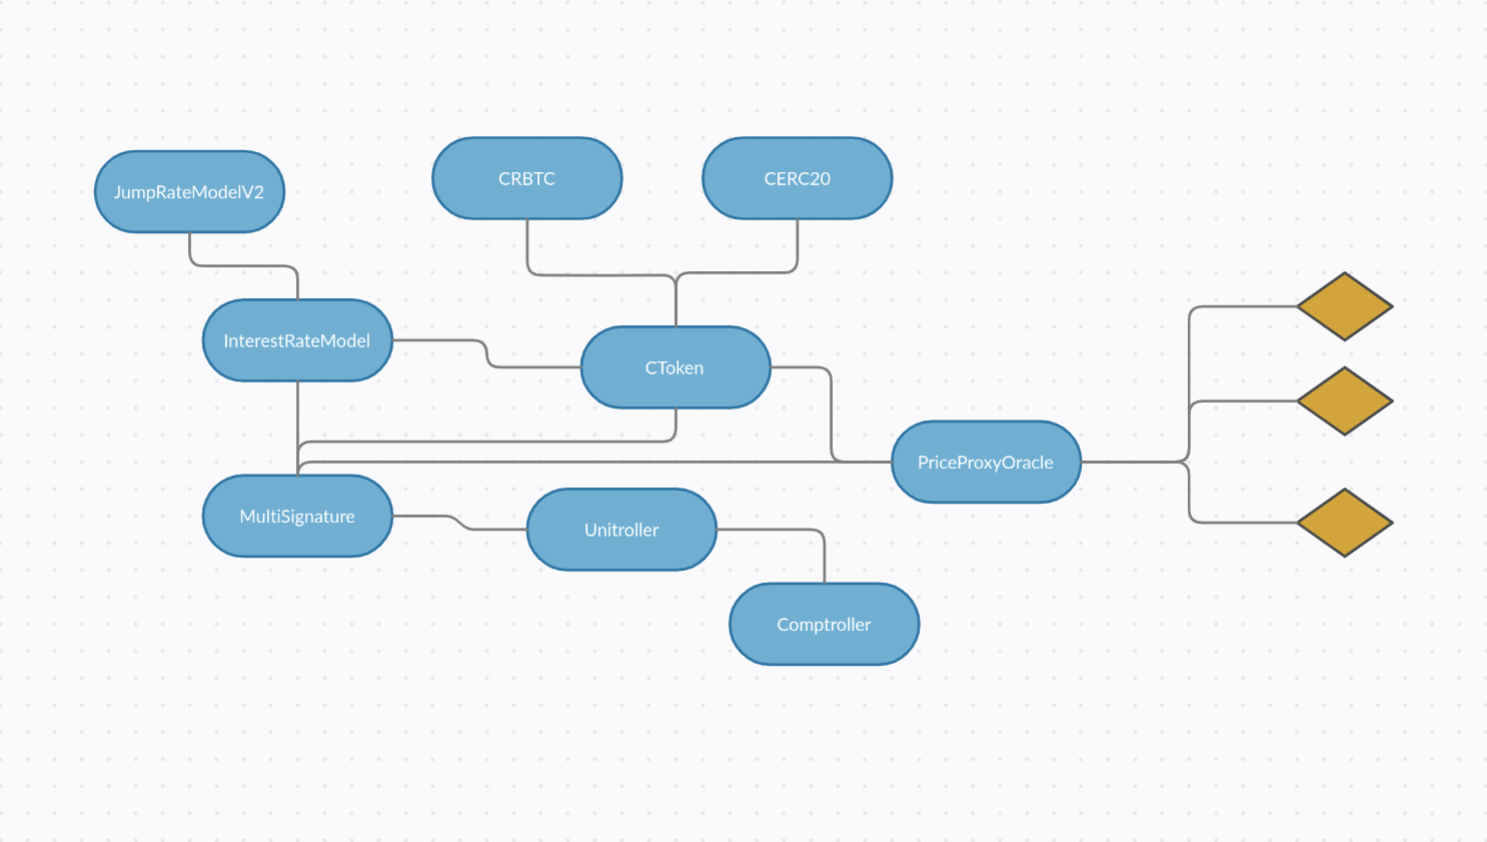
\includegraphics[width=14cm]{contractGraph.png}
\end{center}

%------------------------------------------------
\subsection{CTokens contracts}
At the core of the \textbf{rLending Protocol} are \textbf{cTokens}, identifying each underlying asset supported by the platform.
This section describes the \textit{CToken.sol} contract subsystem and its functionalities.

\begin{itemize}
\item{\textbf{CTokens}} (CErc20.sol and CRBTC.sol)
\end{itemize}

\textbf{cTokens} are self-contained borrowing and lending contracts. \textbf{CToken.sol} contains the core logic. Each \textit{cToken} is assigned an interest rate and risk model (see \textbf{InterestRateModel} and \textbf{Comptroller} sections), and allows accounts to \textit{mint} (supply capital), \textit{redeem} (withdraw capital), \textit{borrow} and \textit{repay a borrow}. Each \textbf{CToken} is an \textbf{ERC-20} compliant token where balances represent ownership of a portion of the liquidity pool (see \textbf{market}).
\\
In other words, since each asset supported by the \textbf{rLending Protocol} is integrated through a \textbf{CToken}, by minting them, users (1) earn interest through the \textbf{cToken's exchange rate}, which increases in value relative to the underlying asset, and (2) gain the ability to use \textbf{cTokens} as collateral for borrowing.\\
\textbf{cTokens} are the primary means of interacting with the Protocol and whenever a user mints, redeems, borrows, repays a borrow, liquidates a borrow, or transfers \textbf{cTokens}, they will do so indirectly using this contract. \\
\\
There are currently two types of \textbf{cTokens}: \textbf{CErc20.sol} and \textbf{CRBTC.sol}. Though both types expose the \textit{EIP-20} interface, \textbf{CErc20.sol} wraps any underlying \textit{ERC-20} asset, while \textbf{CRBTC.sol} simply wraps \textbf{rBTC} (\textit{the base currency within the RSK Network}) itself. As such, the core functions which involve transferring an asset into the protocol have slightly different interfaces depending on the type.

\begin{itemize}
\item \textbf{Comptroller contracts}(Unitroller.sol and Comptroller.sol)
\end{itemize}

This is the risk model system, which validates permissible user actions and disallows actions if they do not fit certain risk parameters. For instance, the Comptroller enforces that each borrowing user must maintain a sufficient collateral balance across all \textit{cTokens}, or else incur in shortfall and becoming prone to liquidation.
\\

\textit{Unitroller} is a proxy contract that controls the storage and admin functions for the latest implementation of \textit{Comptroller}. \textbf{rLending} uses \textbf{ComptrollerG4.sol} which in turn is the contract that updates the \textit{Comptroller}'s risk model system, that keeps track of the listed markets, manages the user's mints and borrows, allowances and market limits.
\\
If a user's borrowing balance exceeds their total collateral value (borrowing capacity) due to the value of collateral falling, or borrowed assets increasing in value, the public \textit{function liquidate()} can be called, which exchanges the invoking user's asset for the borrower's collateral, at a \textit{slightly better}\footnote{see liquidation factor} than market price.
\\
In case you need further information regarding the many roles this subsystem plays, we encourage you to read up on the official rLending documentation\footnote{\href{https://rlending.app/docs}{The official rLending Documentation}}.


\begin{itemize}
\item \textbf{Interest Rate Model subsystem}
\end{itemize}

Markets are defined by an interest rate, applied to all borrowers uniformly, which adjust over time as the relationship between supply and demand changes. The history of each \textit{interest rate}, for each asset market, is captured by an \textbf{Interest Rate Index}, which is calculated each time an interest rate changes, resulting from a user minting, redeeming, borrowing, repaying or liquidating the asset. 
Each time a transaction occurs, the\textbf{Interest Rate Index} for the asset is updated and compounded with the interest since the prior index, using the interest for the period, denominated by $r * t$, calculated using a per-block interest rate:
\begin{center}
$Index_{a,n}= Index_{a,(n-1)}*(1+r*t)$
\end{center}

The market’s total borrowing outstanding is updated to include interest accrued since the last index:

\begin{center}
$totalBorrowBalance_{a,n}= totalBorrowBalance_{a,(n-1)}*(1+r*t)$
\end{center}

And a portion of the accrued interest is retained (set aside) as reserves, determined by a
\textbf{reserveFactor}, ranging from 0 to 1:

\begin{center}
$reserves_{a}= reserves_{a,(n-1)}+ totalBorrowBalance_{a,(n-1)}*(r*t*reserveFactor)$
\end{center}

This way, a borrower's balance, including accrued interest, is simply the ratio of the current index divided by the index when the user's balance was last checkpointed. The balance for each borrower address in the cToken is stored as an account checkpoint. An account's checkpoint is an internal Solidity\footnote{\href{https://docs.soliditylang.org/en/v0.8.1/}{Solidity documentation}} structure describing the balance at the time interest was last applied to that account.
\\ 
\textit{InterestRateModel} is an interface that wraps the different versions of interest models. Each one of them improves on the previous form for calculating borrow and utilization rates. The latest implementation being \textbf{JumpRateModelV2.sol}.


%------------------------------------------------
\subsection{Price Oracle contracts}
This subsystem controls the integration of \textbf{Price Oracle Feeds} for any given market listed in the \textbf{rLending Protocol}. A Price Oracle maintains the current exchange rate of each supported asset while the protocol delegates the ability to set the value of assets to a committee\footnote{\href{https://rlending.app/docs/security}{see Multi-sig contract}} which pools prices from the top exchanges. These exchange rates are used to determine borrowing capacity and collateral requirements. The rates are also used for all functions which require calculating the value equivalent of an account.

\begin{itemize}
\item\textbf{PriceOracleProxy.sol}
\end{itemize}

This contract manages the mapping of the \textit{cTokenAddress} to \textit{adapterAddress}. Through this proxy the protocol abstracts itself from any oracle's interface. Each \textbf{PriceOracleAdapter.sol} implements a specific oracle that is to be included in the mapping, making the oracle's interface code-agnostic from the proxy side.

\begin{center}
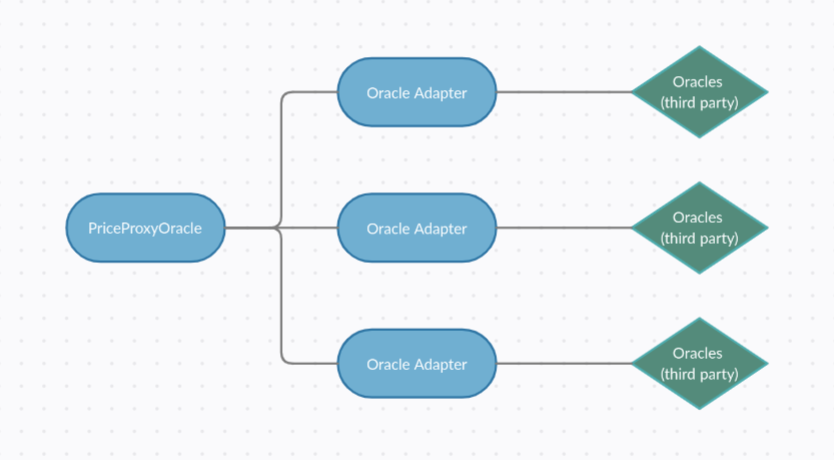
\includegraphics[width=8cm]{oracles.png}
\end{center}

\begin{itemize}
\item\textbf{OracleAdapters Layer}
\end{itemize}

Given that we foresee the posibility of diverse Oracle systems being deployed in the network, we developed a middle-layer contract adapter system to interact with each Oracle as intermediary. This way, the \textbf{rLending Protocol} is capable of receiving price information from every kind of Oracle, regardless of it's implementation.

%------------------------------------------------
\subsection{Gnosis Multisignature Integration}

At launch \textbf{rLending} is relying on \textit{Gnosis Multisig}\footnote{\href{https://github.com/gnosis/MultiSigWallet/blob/master/contracts/MultiSigWallet.sol}{https://github.com/gnosis/MultiSigWallet/blob/master/contracts/MultiSigWallet.sol}} to create a committee of specialists that will manage the protocol's most critical functionalities. After a reasonable time on main-net, we propose moving on to a Governance based schema.\\
This means that the initial \textbf{rLending} deploy will have \textit{admin}/\textit{guardian} addresses pointing to \textit{Gnosis Multisig} contract, that has distributed the capability of updating core values within the protocol:

\begin{itemize}
\item The ability to list a new cToken market
\item The ability to update the interest rate model per market
\item The ability to update the oracle or any adapter address
\item The ability to withdraw the reserve of a cToken
\item The ability to update the Risk model contracts
\item The ability to choose a new admin
\end{itemize}

\begin{center}
\noindent\rule{8cm}{0.4pt}
\end{center}

%----------------------------------------------------------------------------------------
%	CONSIDERATIONS
%----------------------------------------------------------------------------------------
\section{Final notes and considerations}

\begin{itemize}
\item We acknowledge that \textbf{rLending} will launch as a partially decentralized application. As stated in the previous section: the protocol relies on a committee regulating the Gnosis Multi-Signature contracts. After a grace period, the protocol should fully transition to a governance system.
\item Threat models and Security checks, as well as audits for the inherited Compound code, have been reviewed both by the rLending team and third parties with satisfactory results.
\item We strongly encourage inexperienced users to carefuly study \href{https://test.rlending.app/doc}{the documentation} and gain a deep understanding of the risks involved before using the platform.
\item \textbf{rLending} is distributed under \textit{BSD-3 Licence}\footnote{\href{https://github.com/riflending/rlending-protocol/blob/master/LICENSE}{https://github.com/riflending/rlending-protocol/blob/master/LICENSE}}
\\[0.1in]
\end{itemize}
\begin{center}
\noindent\rule{8cm}{0.4pt}
\\[0.5in]
Contact: \href{mailto:support@rlending.app}{support@rlending.app}\\
Git: \href{https://github.com/riflending/rlending-protocol}{github.com/riflending}\\[0.1in]
\textbf{\href{https://test.rlending.app}{Try the rLending Open Beta}}

\end{center}


%----------------------------------------------------------------------------------------

\end{document}
